\documentclass{article}
\usepackage[english, magyar]{babel}
\usepackage[hidelinks]{hyperref}
\usepackage{t1enc}
\usepackage[margin=3cm]{geometry}
\usepackage{graphicx}
\usepackage{float}
\frenchspacing

\begin{document}
	\begin{titlepage}
		\title{\Huge{\textbf{KávéKatt}}\\
				\LARGE{Web Technológiák I.\\beadandó feladat}}
		\author{\Large{\textbf{Készítette}: Martinák Mátyás - KLNSPG}}
		\date{\vspace{390pt}\textbf{Miskolc, 2023}}
		\maketitle
	\end{titlepage}

\tableofcontents
\clearpage

\section{Bevezető}
\indent\indent Ez a feladat \textit{Web Technolóiák I.} tantárgyból készült, és egy egyszerű \textbf{HTML, CSS, JavaScript} weboldalt valósít meg, melynek címe: \textbf{KávéKatt}. A weboldal egy kávézó bemutatkozó weboldala. Az oldal modern technológiákat és megoldásokat alkalmaz, mint például az animációk, reszponzív dizájn és kliensoldali űrlapellenőrzés.

A weboldal elsődleges célja, hogy a látogatókat tájékoztassa a kávézó történetéről, aktuális kínálatáról és eseményeiről. Ezen túlmenően az oldal egy olyan platformot kínál, ahol a látogatók egyszerűen foglalhatnak asztalt, elkerülve a hagyományos telefonos foglalás során tapasztalható kellemetlenségeket.

A KávéKatt weboldala modern technológiák segítségével készült. A strukturális felépítésért az HTML (HyperText Markup Language) felel, míg a vizuális megjelenítésért a CSS (Cascading Style Sheets). Az interaktív funkciókért, mint például az űrlapok validálása, a JavaScript programozási nyelv felelős.

\section{HTML struktúra és tartalmi felépítés}
\subsection{Oldalak leírása}
\indent\indent A Főoldal egy meleg üdvözlő szöveggel ("Üdvözlünk a KávéKatt kávézóban!") fogadja a látogatókat. Itt megtalálható egy navigációs menü, amely segítségével könnyedén navigálhatunk a weboldal további részei között, mint például a Történet, Galéria és Asztalfoglalás oldalak. A főoldal központi részén egy képet láthatunk a kávézó napi kínálatáról, mellyel az élményt egy rövid képaláírás ("Üdvözöljük a KávéKatt-nál, ahol a kávé mindig friss és finom!") teszi teljessé.

A Történetünk oldalon a látogatók betekintést nyerhetnek a kávézó múltjába. A fejlécben található "Történetünk" cím alatt olvasható egy rövid összefoglaló a kávézó történetéről, amelyben kiemelik a fontosabb eseményeket és a kávézó különlegességeit. A történet számos fontos mérföldkövet tartalmaz, például a kávézó megnyitását vagy saját kávémárka bevezetését.

A Galéria oldal a vizuális élményekre koncentrál. Itt a látogatók képeken keresztül ismerkedhetnek meg a kávézó hangulatával. A képeket egy átlátható, két oszlopos táblázatban rendezik, ahol minden képhez tartozik egy rövid leírás, hogy a látogatók tudják, mit is látnak pontosan.

Végül, de nem utolsósorban, az Asztalfoglalás oldalon a látogatók gyorsan és egyszerűen foglalhatnak asztalt a kávézóban. Az űrlap tartalmazza az összes szükséges mezőt az asztalfoglaláshoz, például a név, kívánt kávéfajta, cukor típusa, asztal dekorációjának színe és a foglalás dátuma. Emellett az oldal stílusos hibakezelési funkciókat is tartalmaz, hogy a felhasználók azonnali visszajelzést kapjanak a beírt információkról.
\subsubsection{Főoldal}
\begin{enumerate}
	\item \textbf{Dokumentum Típusa}: A \textbf{<!DOCTYPE html>} jelzi, hogy a dokumentum egy HTML5 dokumentum.
	\item \textbf{Fejléc (head)}:
		\begin{itemize}
			\item \textbf{'charset'} és \textbf{'viewport'} meta elemek: Ezek az oldal karakterkódolását és reszponzivitását adják meg.
			\item A \textbf{cím (title)} beállítja az oldal címét: "KávéKatt".
			\item \textbf{Stílus és script linkelése}: A CSS fájl (style.css) és a jQuery, valamint a script.js linkelve van az oldalhoz.
		\end{itemize}
	\item \textbf{Törzs (body)}:
		\begin{itemize}
			\item \textbf{Fejléc (header)}: Egy \textbf{'h1'} címmel köszönti a látogatókat.
			\item \textbf{Navigációs menü (nav)}: Egy \textbf{'ul'} listával rendelkező menü az oldal különböző részeihez való navigációhoz.
			\item \textbf{Képaláírás}: Egy 'span' elem tájékoztat az új kínálatakról.
			\item \textbf{Kép}: Egy táblázatban egy kép található a napi kávéval.
		\end{itemize}
\end{enumerate}
\begin{figure}[H]
	\centering
	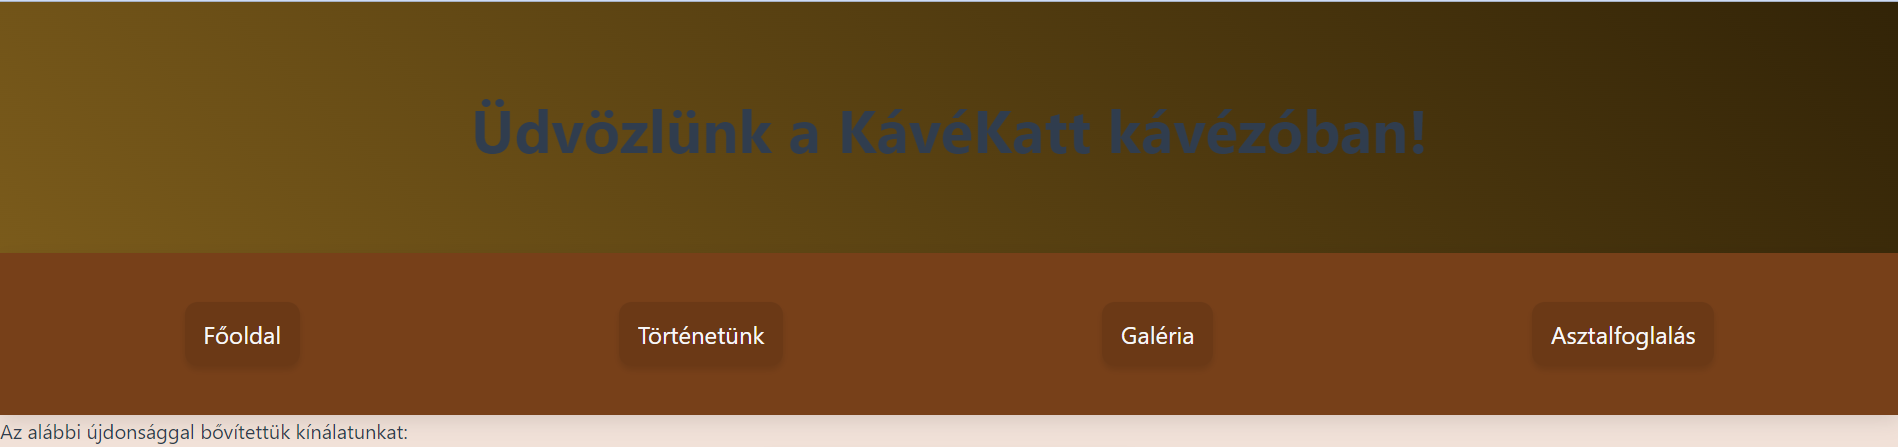
\includegraphics[width=0.9\linewidth]{kvkatt.png}
	\caption{A kezdőlap és a navigációs bar}
	\label{fig:index}
\end{figure}
\begin{figure}[H]
	\centering
	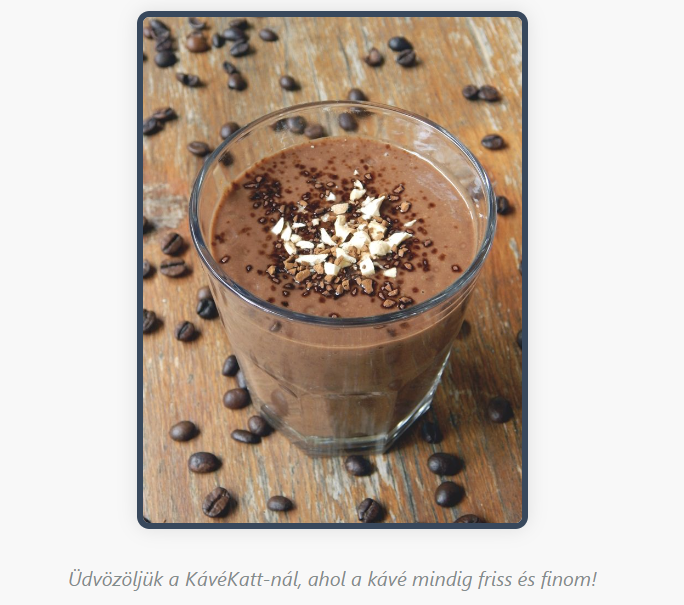
\includegraphics[width=0.6\linewidth]{kv.png}
	\caption{A nap kávéja}
	\label{fig:indexkv}
\end{figure}
\subsubsection{Történetünk}
\begin{enumerate}
	\item \textbf{Fejléc (head)}: Az alapvető meta elemek és a CSS fájl linkelése, hasonlóan az előző oldalhoz.
	\item \textbf{Törzs (body)}:
		\begin{itemize}
			\item \textbf{Fejléc (header)}: Egy \textbf{'h1'} címmel jelzi az oldal tartalmát.
			\item \textbf{Navigációs menü (nav)}: Ugyanaz a navigációs menü, mint a Főoldalon.
			\item \textbf{Történet összefoglaló}: Egy \textbf{'span'} elemmel és egy paragrafussal (p) ismerteti a kávézó történetét.
			\item \textbf{Kiemelt események}: Egy \textbf{'table'} táblázatban sorolja fel a kávézó fontosabb eseményeit.
		\end{itemize}
\end{enumerate}
\begin{figure}[H]
	\centering
	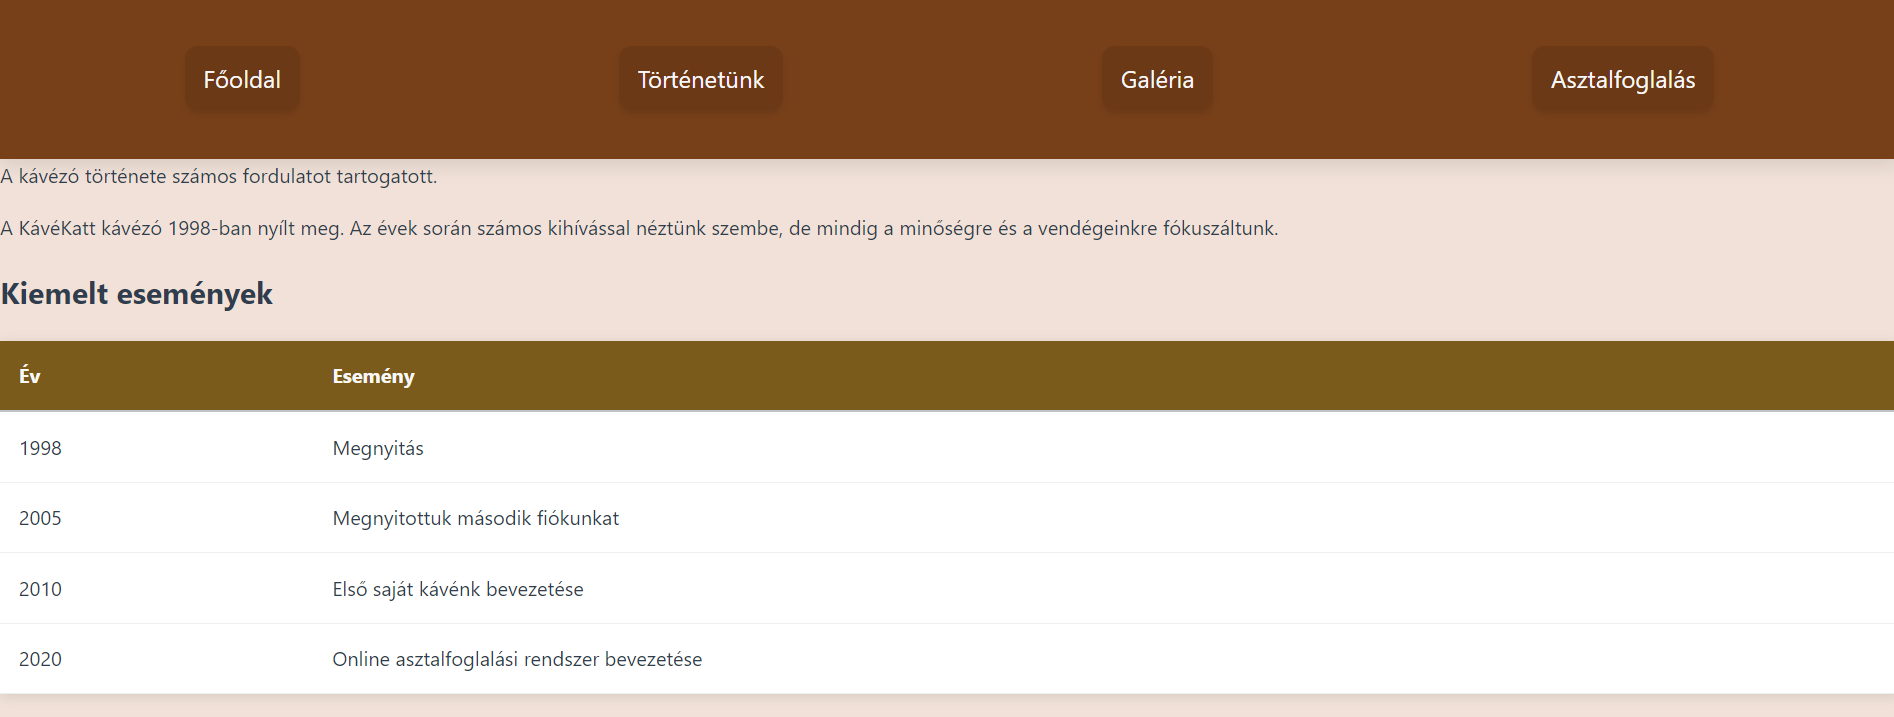
\includegraphics[width=0.9\linewidth]{story.png}
	\caption{A "Történetünk" oldal}
	\label{fig:story}
\end{figure}
\subsubsection{Galéria}
\begin{enumerate}
	\item \textbf{Fejléc (head)}: Az alapvető meta elemek és a CSS fájl linkelése, hasonlóan az előző oldalhoz.
	\item \textbf{Törzs (body)}:
		\begin{itemize}
			\item \textbf{Fejléc (header)} és \textbf{Navigációs menü (nav)}: Ugyanazok, mint az előző oldalakon.
			\item \textbf{Képaláírás}: Egy \textbf{'span'} elem tájékoztat a képgaléria tartalmáról.
			\item \textbf{Képgaléria}: Egy \textbf{'div'} tartalmaz egy táblázatot, amelyben képek (img elemek) vannak, mindegyikhez egy rövid leírással.
		\end{itemize}
\end{enumerate}
\begin{figure}[H]
	\centering
	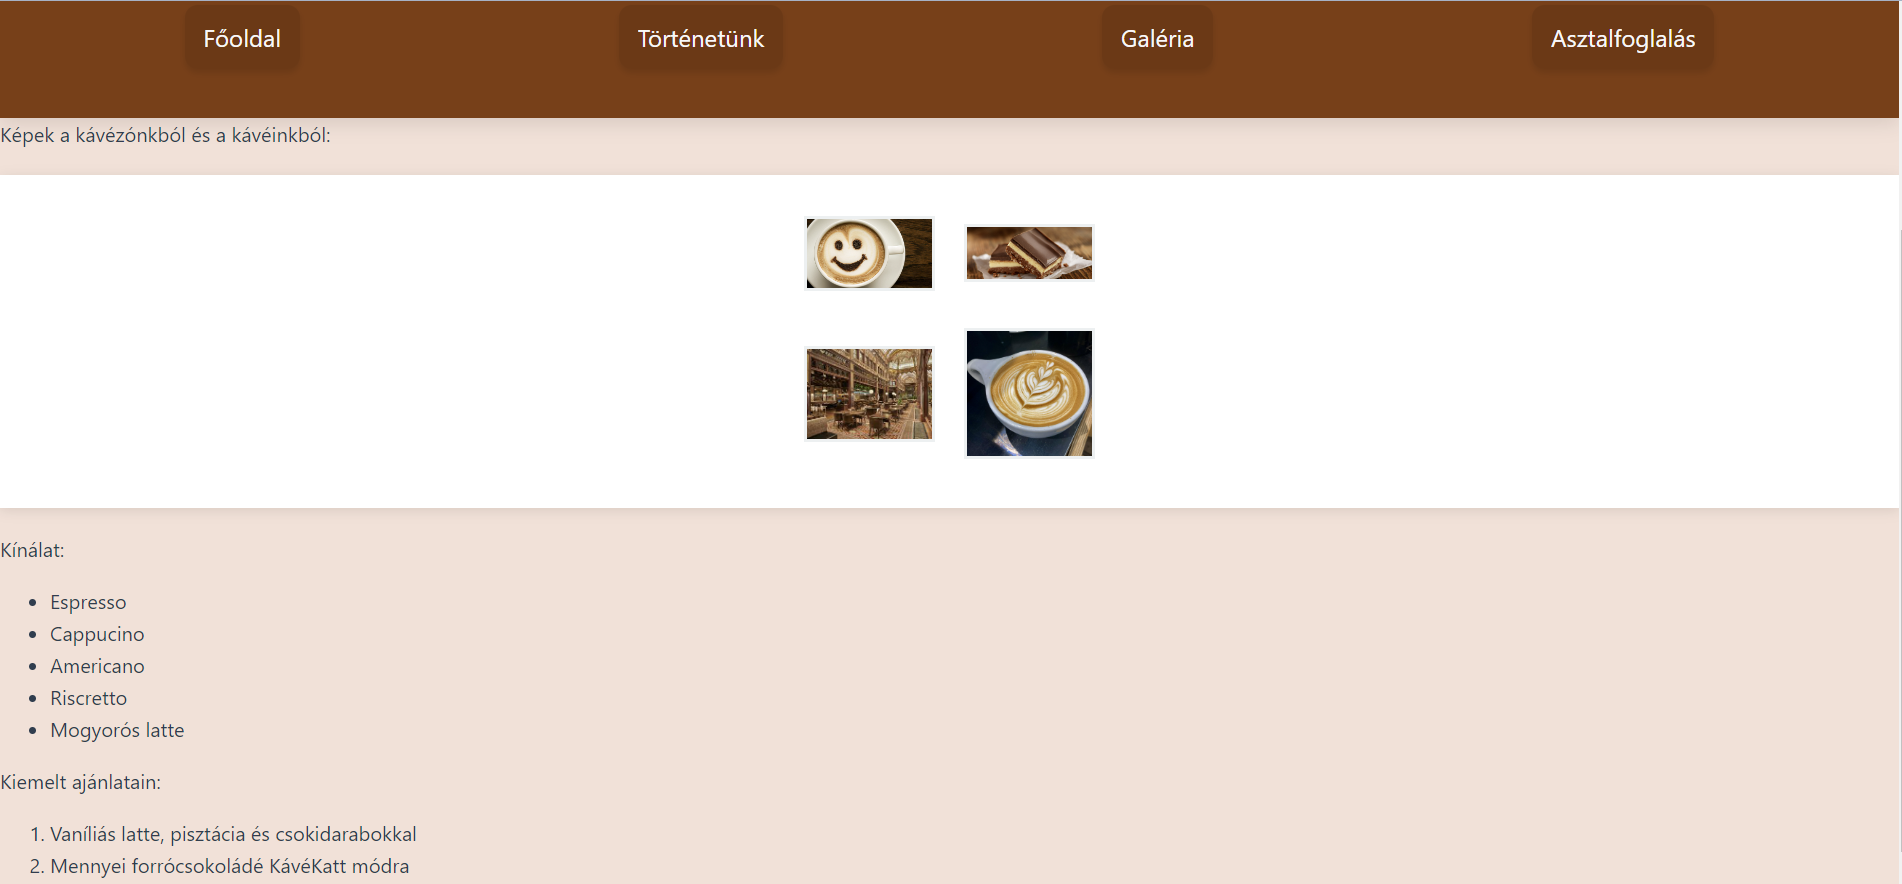
\includegraphics[width=0.9\linewidth]{gallery.png}
	\caption{A "Galéria" oldal}
	\label{fig:gallery}
\end{figure}
\clearpage

\subsubsection{Asztalfoglalás}
\begin{enumerate}
	\item \textbf{Fejléc (head)}: Az alapvető meta elemek, CSS, és a jQuery, valamint a script.js linkelése.
	\item \textbf{Törzs (body)}:
		\begin{itemize}
			\item \textbf{Fejléc (header)} és \textbf{Navigációs menü (nav)}: Hasonlóan az előző oldalakhoz.
			\item \textbf{Stílus}: Helyben definiált CSS stílusok az űrlap hibaüzeneteihez.
			\item \textbf{Foglalási űrlap}: Egy \textbf{'form'} elem, amely különböző beviteli mezőket tartalmaz, mint szövegbevitel, rádiógombok, jelölőnégyzetek, színválasztó és dátumválasztó. Ezenkívül tartalmaz egy "Foglalás" nevű elküldő gombot is.
		\end{itemize}
\end{enumerate}
\begin{figure}[H]
	\centering
	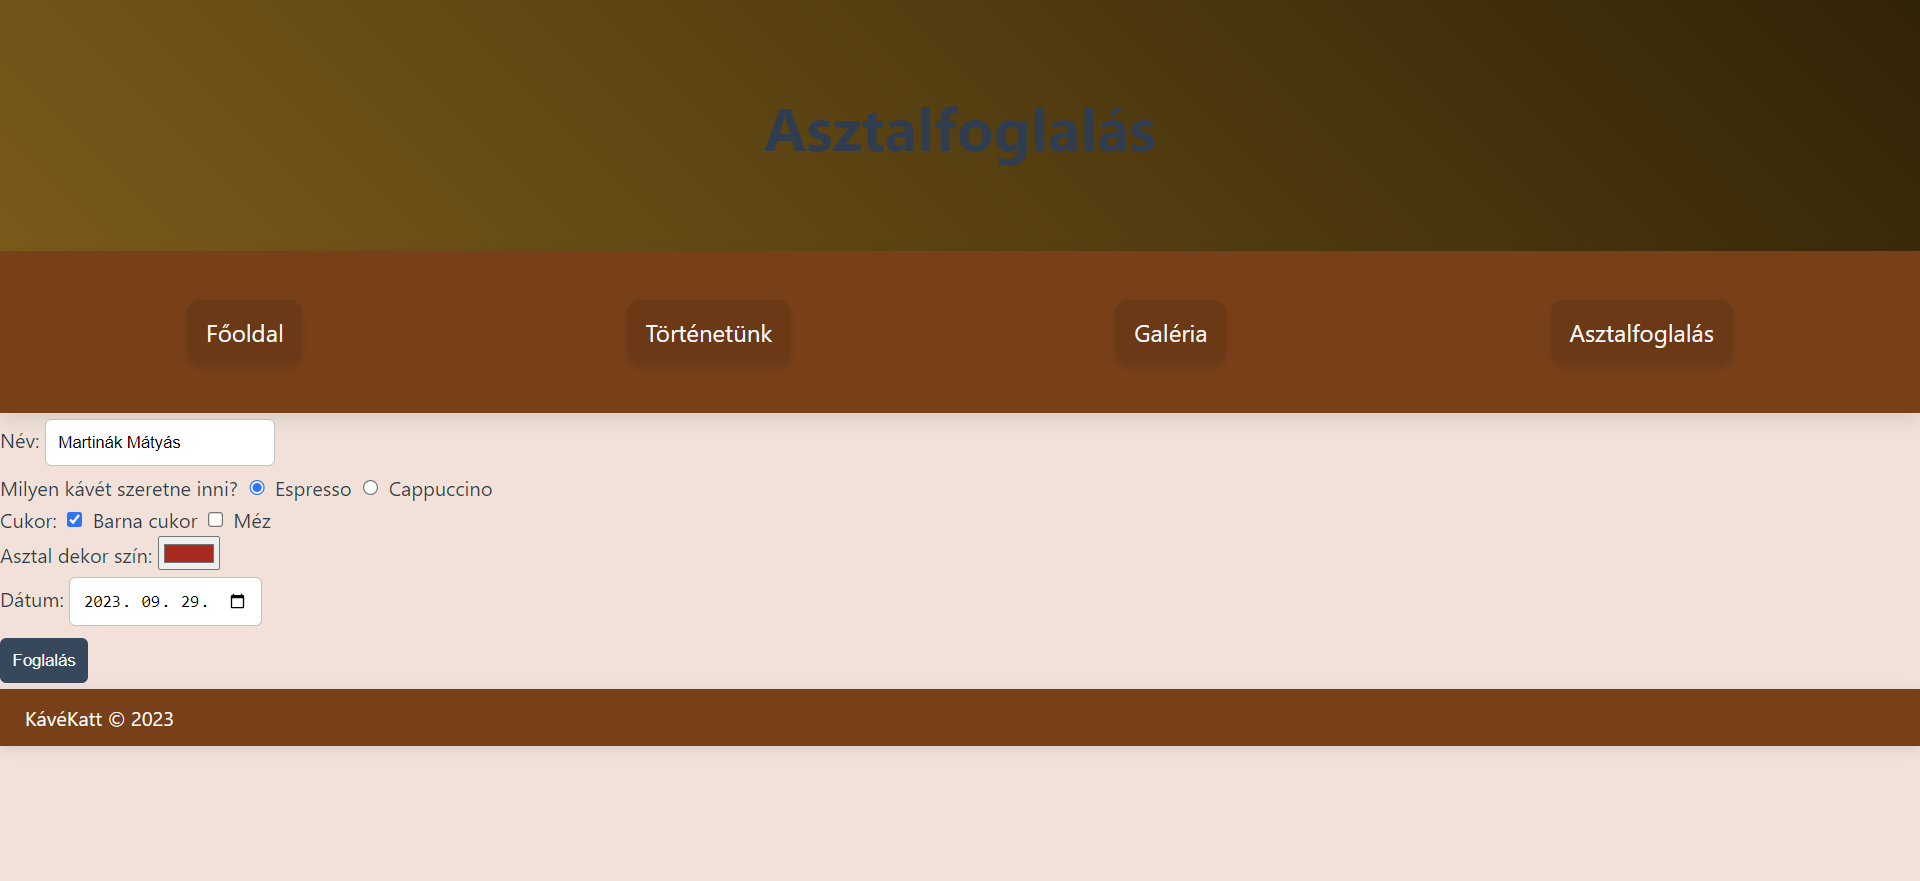
\includegraphics[width=0.9\linewidth]{form.png}
	\caption{Az "Asztalfoglalás" oldal, űrlappal kitöltve}
	\label{fig:form}
\end{figure}
\section{CSS formázás és design irányelvek}
\indent\indent A weboldal alapvető dizájnjában a body az előre definiált 'Segoe UI', Tahoma, Geneva, Verdana és sans-serif betűtípusok egy kombinációját alkalmazza. A háttérszín egy finom bézs árnyalatot (\#f4e0d7) kapott, míg az alapértelmezett szövegszín sötétkék (\#2c3e50). A sormagasság (line-height) 1.6-ra lett állítva a jobb olvashatóság érdekében.

A weboldal fejlécében (header) a háttér egy 45 fokos szögben elhelyezkedő lineáris gradient, ami egy barna árnyalatból (\#805900) egy sötétbarna (\#352301) árnyalatba megy át. Ez a háttér a felhasználói interakció során változhat; amikor a kurzorral a fejléc fölé hozakodunk, az árnyalatok világosodnak és a barna színek élénkebbé válnak.

A navigációs menü (nav) és a lábléc (footer) egy mély barna színű háttérrel rendelkezik. Az ezeken a területeken található szövegek színe szürkés-fehér (\#f8f8f8). A navigációs menü a felhasználó számára könnyen navigálható, hiszen a linkek világos hátteret és árnyékolást kaptak a kiemelés érdekében. Ha rákattintunk egy linkre, annak a háttere sötétedik, ezzel is jelezve, hogy az adott oldalon vagyunk.

A weboldalon található galéria stílusa korszerű, a képek flexibilis elrendezésben jelennek meg, lehetővé téve az optimális térkihasználást. A bélyegképek, amik a galériában jelennek meg, szélesebb kerettel rendelkeznek a többi képhez képest, így azok kiemelkednek.

A weboldal interaktív elemeinél, mint például a beviteli mezőknél és gomboknál, az egyszerűség és a felhasználói élmény volt a fő szempont. A gomboknak és beviteli mezőknek sima átmenetei vannak, valamint az aktív vagy hibás mezők azonnal felismerhetőek a színelméleteknek köszönhetően.

Végül, de nem utolsósorban, az oldalon található képtáblázat és a képaláírások speciális stílussal rendelkeznek, így azok is egyediek és könnyen felismerhetőek.

Összefoglalva, a CSS kód gondosan megtervezett és a modern webdesign elvárásainak megfelelően lett összeállítva, garantálva a felhasználók számára az intuitív és kellemes böngészési élményt.
\section{JavaScript és Interaktivitás}
\indent\indent Miután a weboldal összes eleme teljesen betöltődött, a kód beállítja az alapvető változókat, hogy hozzáférhessen bizonyos HTML elemekhez. Először is, megtalálja és tárolja az "urlapForm" azonosítójú űrlapot a form változóban. Ezen kívül kiválaszt egy input mezőt az "nev" azonosítóval, és ezt tárolja a nev változóban.

Ezután létrehoz egy új 'span' elemet a nevError változóban, amelyet a hibaüzenetek megjelenítésére szán. Ennek az új span elemnek az azonosítója "nev-error", és a "error-message" osztályba tartozik. Ez a span elem közvetlenül a név input mező után kerül elhelyezésre.

A kód további részei körül vannak az űrlap validálásával. Egy showError nevű funkciót használ, hogy animált módon jelenítse meg a hibaüzeneteket. Amikor ezt a funkciót meghívják, a hibaüzenet először átlátszó lesz, majd néhány milliszekundumon belül láthatóvá válik, így az animáció hatásosabbnak tűnik a felhasználó számára.

Amikor a felhasználó megpróbálja elküldeni az űrlapot, a kód ellenőrzi a következőket: van-e megadva név az input mezőben; kiválasztottak-e egy kávét a kávé választókból; és megadott-e egy dátumot. Ha valamelyik feltétel nem teljesül, a hibaüzenetek megjelennek, és az űrlap elküldése megakadályozódik.

A kód befejezéseként néhány további elemet is kiválaszt a dokumentumból, így azokkal később manipulációt végezhet, illetve létrehoz egy új "footer" elemet "KávéKatt © 2023" felirattal, és hozzáadja a weboldalhoz.

\begin{figure}[H]
	\centering
	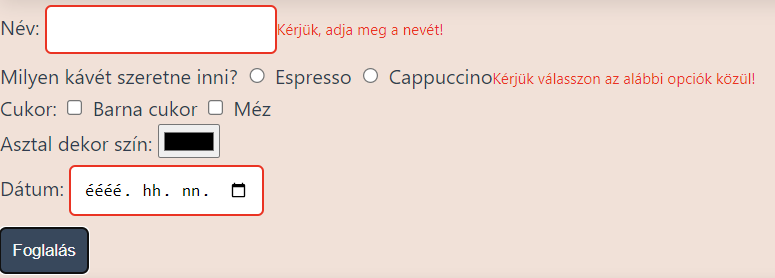
\includegraphics[width=0.8\linewidth]{badform.png}
	\caption{A űrlap helytelenül kitöltve}
	\label{fig:badform}
\end{figure}
\clearpage

\section{Összefoglalás}
A bemutatott kódok egy egyszerű, de jól strukturált weboldalt formálnak, melynek alapvető célja, hogy a felhasználó be tudja adni bizonyos adatait egy űrlapon keresztül, valamint megjelenítse az oldal stílusos kinézetét.

\noindent \textbf{HTML}: Az oldal struktúrája egy fejlécet, navigációs menüt, galériát, egy űrlapot és láblécet tartalmaz. A galéria különböző képekből áll, amelyek miniatűrök formájában jelennek meg. Az űrlap segítségével a felhasználó megadhatja a nevét, kiválaszthat egy kávéfajtát, és megadhat egy dátumot.

\noindent \textbf{CSS}: A stíluslap a modern dizájnelvekhez igazodva biztosítja az oldal vizuális megjelenését. A háttérszín meleg és barátságos, míg a betűk és egyéb elemek árnyékolása apró, de hatásos részletességet ad az oldalnak. A fejléc és a navigációs menü interaktív, átmeneti effektusokkal rendelkezik, amelyek reagálnak a felhasználói interakciókra. Az űrlap elemek jól elkülönülnek, és a hibaüzenetek esetén piros színnel emelkednek ki.

\noindent \textbf{JavaScript}: A JS kód az űrlap validálására koncentrál. Amikor a felhasználó megpróbálja elküldeni az űrlapot, a kód ellenőrzi, hogy a szükséges mezők ki vannak-e töltve. Ha nem, hibaüzeneteket jelenít meg, melyek animáltan tűnnek fel, növelve a felhasználói élményt. Ezen felül az űrlap elküldése megakadályozódik, ha valamelyik mező nem felel meg a kritériumoknak. A kód végén egy láblécet is hozzáad az oldalhoz, ami az oldal tulajdonosának vagy vállalatának az aláírása lehet.
\end{document}